\subsection{Making your first simulation}

Click on the $new~simulation$ button.  This will bring up the new simulation window (see figure \ref{fig:new_new}). From this window double click on the $Organic~Solar~Cells$ icon. This will bring up a sub menu of different types of Organic Solar cells (see figure \ref{fig:new_opv}). The majority of these device simulations have been published in papers and calibrated to real organic solar cells. The oldest is the (non-inverted) P3HT:PCBM device from 2012 \cite{mackenzie2012extracting} and the newest are the PM6:Y6 devices from 2022 \cite{zhu2022single,wopke2022traps}. \emph{Double click on the P3HT:PCBM simulation for this example and save the new simulation to disk.}

Once you have saved the simulation, the main OghmaNano simulation window will be brought up (see figure \ref{fig:simpleinterface}). You can look around the structure of the solar cell, by dragging the picture of the solar cell with your mouse.  Try pressing on the buttons beneath the red square, they will change the orientation to the \emph{xy}, \emph{yz} or \emph{xz} plane. Notice the x,y,z origin marker in the bottom left of the 3D window. The icon with four squares will give you an orthographic view of the solar cell.


Click on the button called \emph{Run simulation}, to run the simulation (hint it looks like a blue play button and is located in the \emph{file} one to the right of the "Simulation type ribbon" ).  The function key F9 will also run the simulation. On slower computers it could take a while. Once the simulation is done, click on the $Output$ tab (see figure \ref{fig:output}), there you will see a list of files the simulation has written to disk.

\noindent
\begin{minipage}{0.45\textwidth}
\centering
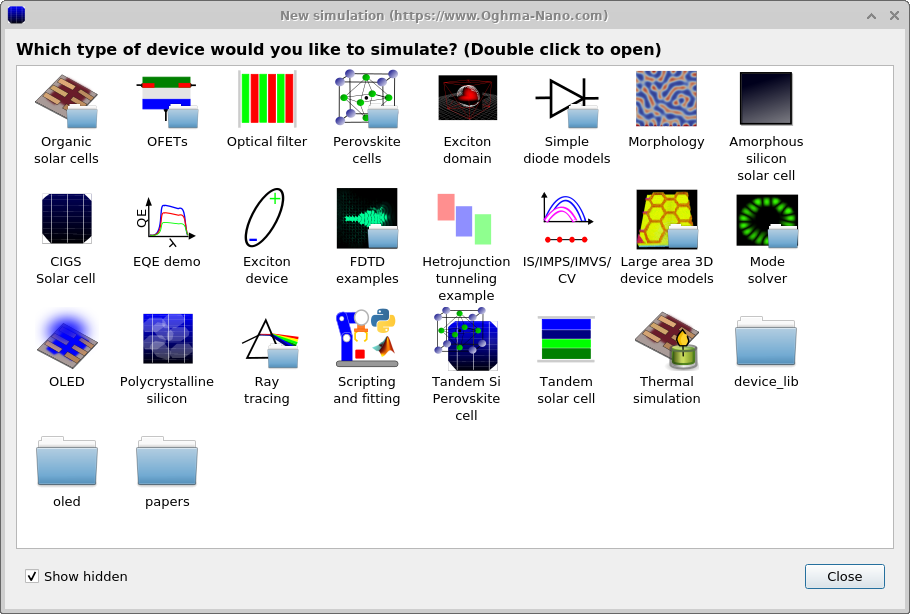
\includegraphics[width=\textwidth,height=0.7\textwidth]{./images/running/new.png}
\captionof{figure}{New simulation window, from here you can select different example simulations. It is often easier to start from a base simulation rather than build your own from scratch.}
\label{fig:new_new}
\end{minipage}
\hspace*{10px}
\begin{minipage}[]{0.45\linewidth}
\centering
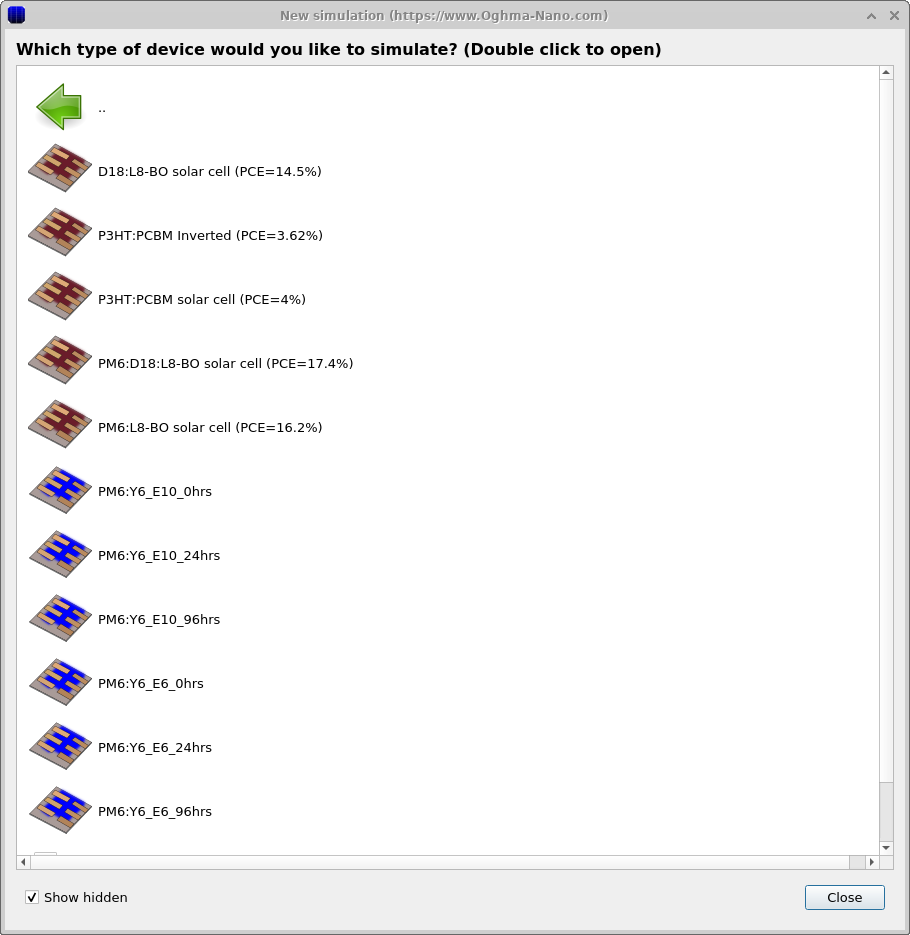
\includegraphics[width=\textwidth,height=0.7\textwidth]{./images/running/new_opv_device.png}
\captionof{figure}{The organic solar cell sub menu. There are quite a few examples of organic solar cells in this menu. The majority of simulations have been used to produce papers \cite{mackenzie2012extracting,zhu2022single,wopke2022traps}.}
\label{fig:new_opv}
\end{minipage}


\subsubsection{What's the best place to save your simulation?}
OghmaNano dumps a lot of data to disk, I therefore recommend you save the simulation to a local disk such as the C:\textbackslash drive, a network drive or USB stick drive will be far too slow for the simulation to run.  I would also not save the simulation onto OneDrive or Dropbox as they are also too slow and saving it there will generate a lot of network traffic.  If you are a power user doing a lot of fitting of experimental data I would also recommend (at your own risk(!)) disabling any extra antivirus software you have installed, as quite often the antivirus software can't keep up with the read/writes to disk.

\begin{figure}[H]
\centering
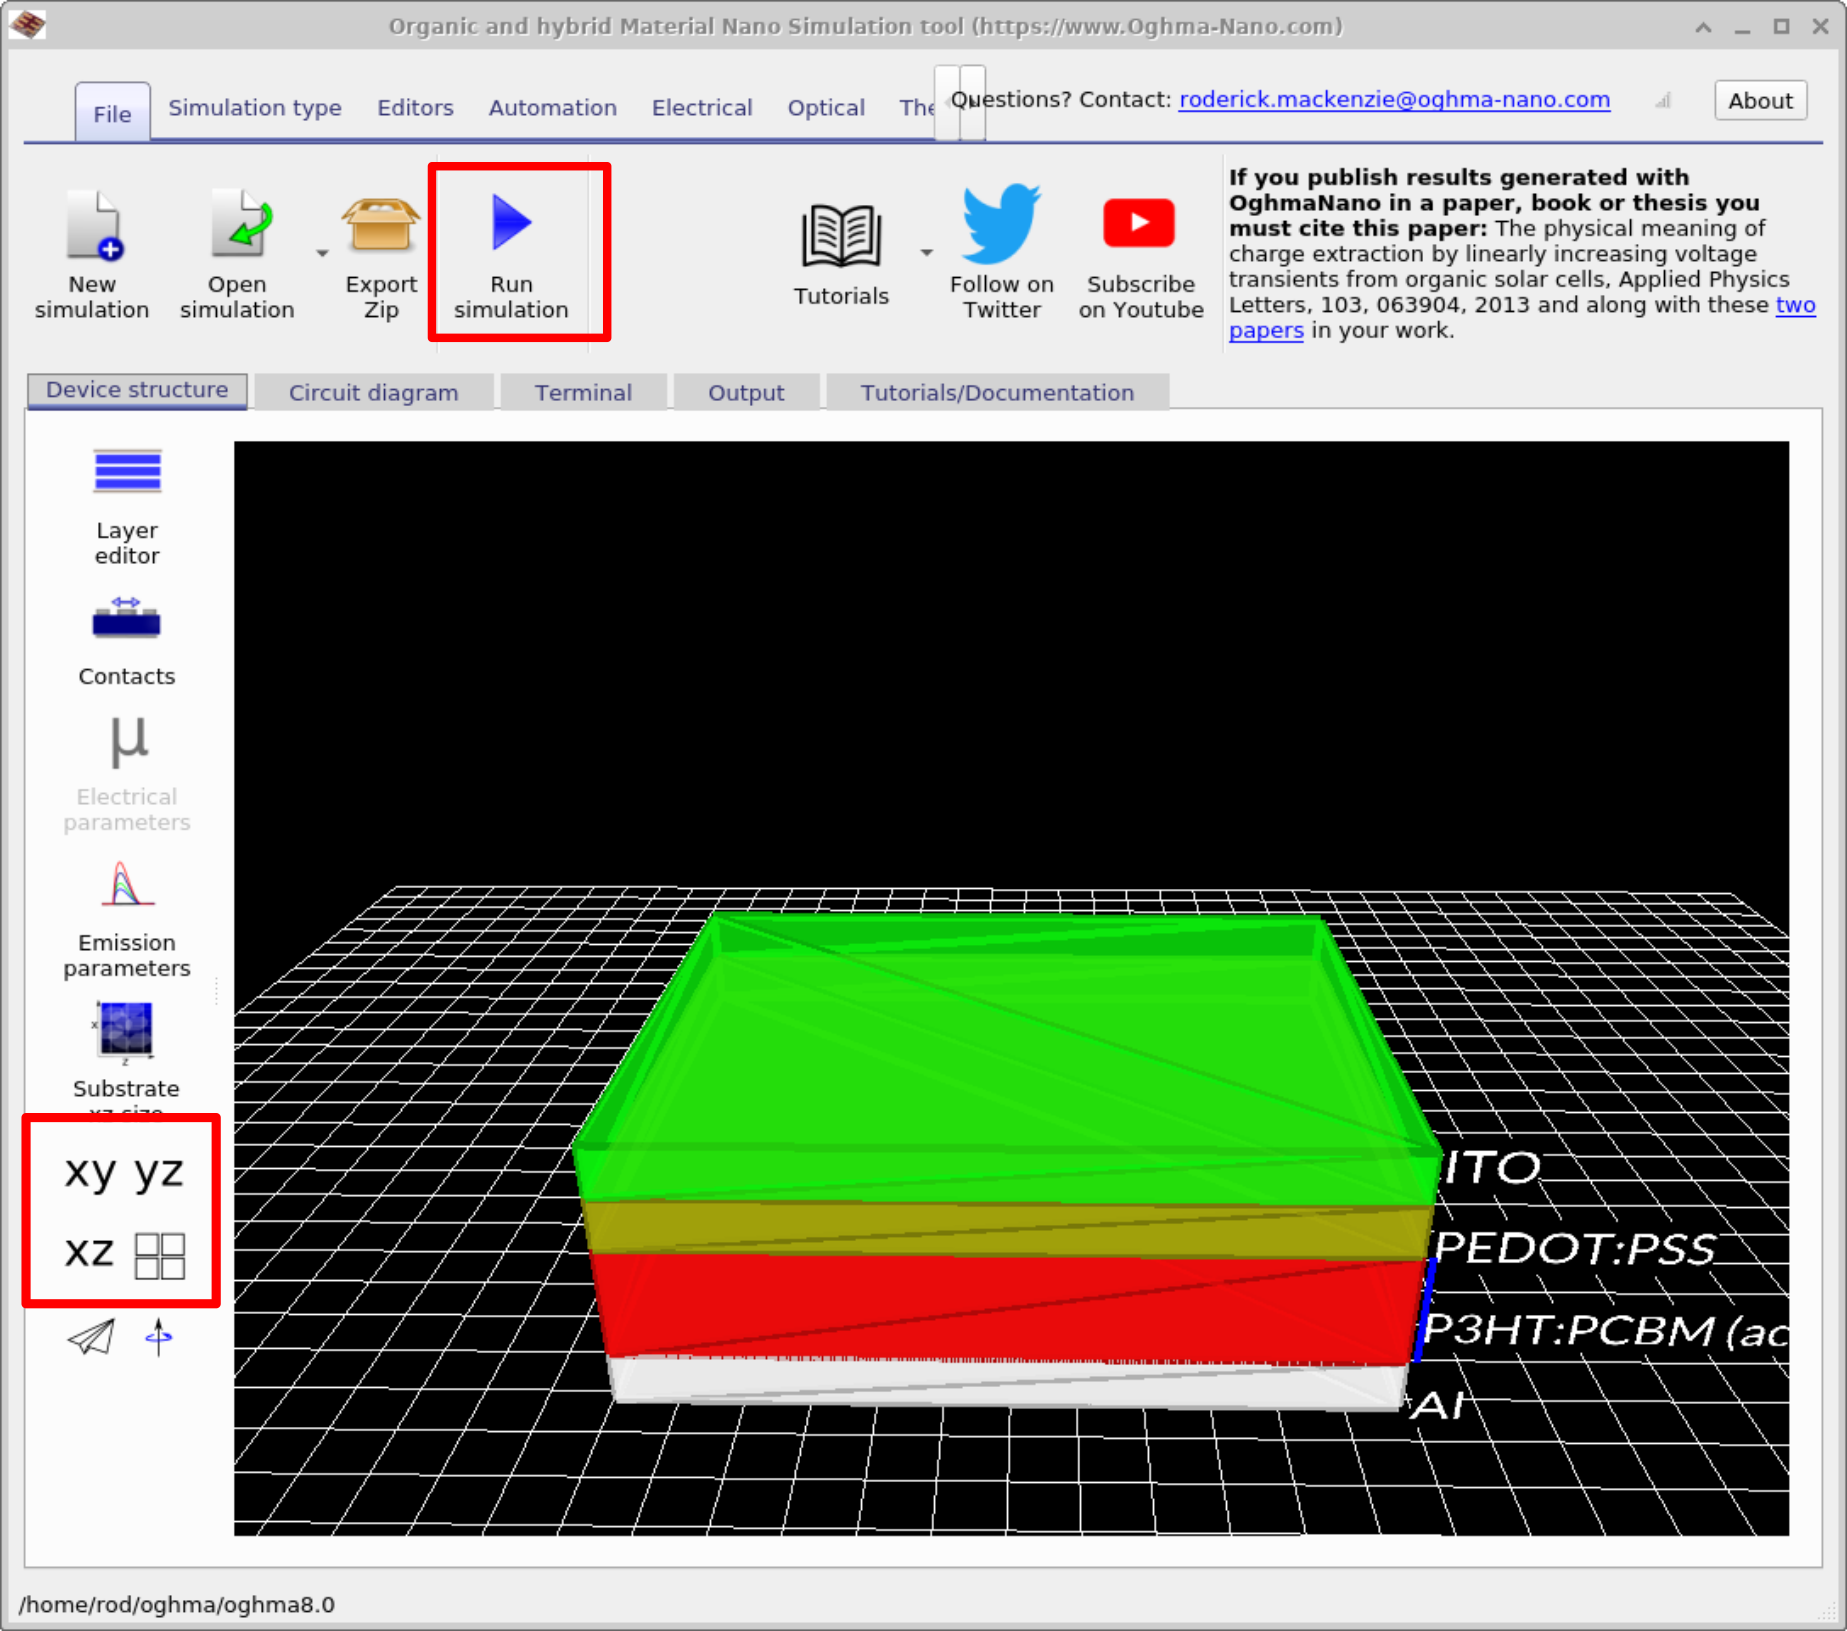
\includegraphics[width=0.8\textwidth,height=0.5\textwidth]{./images/running/simple_interface.png}
\caption{The main OghmaNano simulation window with the xy, yz and xz buttons visible. The play button is also visible which is used to run the simulation, the function key F9 can also be used to run the simulation.}
\label{fig:simpleinterface}
\end{figure}





